%%%%%%%%%%%%%%%%%%%%%%%%%%%%%%%%%%%%%%%%%%
%		Institut d'Optique Graduate School
%%%%%%%%%%%%%%%%%%%%%%%%%%%%%%%%%%%%%%%%%%
%	Interface de pilotage - Aberration 	
%%%%%%%%%%%%%%%%%%%%%%%%%%%%%%%%%%%%%%%%%%
%
% Created by:
%	Julien VILLEMEJANE - 18/june/2025
%	
%
%%%%%%%%%%%%%%%%%%%%%%%%%%%%%%%%%%%%%%%%%%
% Professional Newsletter Template
% LaTeX Template
% Version 1.0 (09/03/14)
%
% Created by:
% Bob Kerstetter (https://www.tug.org/texshowcase/) and extensively modified by:
% Vel (vel@latextemplates.com)
% 
% This template has been downloaded from:
% http://www.LaTeXTemplates.com
%
% License:
% CC BY-NC-SA 3.0 (http://creativecommons.org/li censes/by-nc-sa/3.0/)
%
%%%%%%%%%%%%%%%%%%%%%%%%%%%%%%%%%%%%%%%%%

\documentclass[a4paper,11pt,twoside]{book} % The default font size is 10pt; 11pt and 12pt are alternatives

%%%%%%%%%%%%%%%%%%%%%%%%%%%%%%%%%%%%%%%%%%%%%%%%%%%%%%%%%%%%%%%%%%%%%%%%%%%%%%%%%%%%%%%%%%%%%%%%%%%%%%%%%%%%%%%%%%%%%%%%%%%%%%%%%%%%%%%%%%%%%%%%%%%%%%%%%%%%%%%%%%%%%%%%%%%%%%%%%%%%%%%%%%%%%%%%%%%%%%%%%%%%%%%%%%%%%%%%%%%%%%%%%%%%%%%%%%%%%%%%%%%%%%%%%%%%
\usepackage{tp_villemejane}


%%%%%%%%%%%%%%%%%%%%%%%%%%%%%%%%%%%%%%%%%%%%%%%%
%%%%%%%%%%%%%%%%%%%%%%%%%%%%%%%%%%%%%%%%%%%%%%%%
%%%%%%%%%%%%%%%%%%%%%%%%%%%%%%%%%%%%%%%%%%%%%%%%
%%%%%%%%%%%%%%%%%%%%%%%%%%%%%%%%%%%%%%%%%%%%%%%%
\begin{document}



% Page de garde
\begin{titlepage}

\begin{center}
	\begin{minipage}{2.5cm}
	\begin{center}
		
\includegraphics[width=8cm]{images/Logo-LEnsE.png}
	\end{center}
\end{minipage}\hfill
\begin{minipage}{10cm}
	\begin{center}
	\textbf{Institut d'Optique Graduate School }\\[0.1cm]
    \textbf{Interface Aberrations / Zygo}


	\end{center}
\end{minipage}\hfill


\vspace{5cm}


{\huge \bfseries \textsc{Interféromètre de ZYGO}} \\[0.5cm]
{\large \bfseries Contrôles interforémétriques / Aberrations} \\[0.2cm]

\vspace{2cm}
% Title
\rule{\linewidth}{0.3mm} \\[0.4cm]
{ \huge \bfseries\color{violet_iogs} Notice d'utilisation \\[0.4cm] }
\rule{\linewidth}{0.3mm} \\[1cm]

\vfill

% Bottom of the page
%{\textbf{\large {Année universitaire} 2024-2025}}

\textit{Ce document est disponible au format électronique sur le site du LEnsE - https://lense.institutoptique.fr/ dans la rubrique ???.}

\end{center}
\end{titlepage}

% ----- DEUXIÈME PAGE (sans numérotation) -----
\clearpage
\thispagestyle{empty}
\mbox{} % page vide ou mettre du texte si souhaité

% ----- TROISIÈME PAGE (début de la numérotation à 1) -----
\clearpage
\setcounter{page}{1} % on commence la numérotation ici
\pagenumbering{arabic} % pour utiliser les chiffres arabes
\pagestyle{plain} % ou autre style si souhaité

\begin{minipage}[c]{.25\linewidth}
	
\includegraphics[width=5cm]{images/Logo-LEnsE.png}
\end{minipage} \hfill
\begin{minipage}[c]{.4\linewidth}

\begin{center}
\vspace{0.3cm}
{\Large \textsc{Interféromètre de ZYGO}}

\medskip

\textbf{\Large Notice d'utilisation}

\end{center}
\end{minipage}\hfill

L'\textbf{interférométrie} est couramment utilisée pour \textbf{caractériser la qualité de composants optiques}
usuels (lames à faces parallèles, miroirs plans, miroirs de télescope, systèmes optiques...).

La qualité d'un système optique est caractérisée par l'écart entre sa surface d'onde réelle dans la pupille de sortie du système et la surface d'onde souhaitée. Il est également possible d'en analyser ses aberrations géométriques (coma, astigmatisme, aberration sphérique...).


\section{Interféromètre de Zygo}

Le \textbf{ZYGO} est un \textbf{interféromètre laser} de type Fizeau (par division d'amplitude) équipé d'un système de décalage de phase. Il permet des mesures de surfaces d'onde aberrantes de l'ordre de $\lambda/10$ (PV). L'analyse du front d'ondes se fait par décalage de phase.

Les \textbf{interféromètres de ZYGO} (ou Zygoto) utilisent un Laser \textit{Helium Néon} (HeNe) de longueur d'onde de $632.8\operatorname{nm}$, monomode, de très grande longueur de cohérence. Un système d'épuration laser suivi d'un système de lentille permet d'obtenir un faisceau uniforme et parfaitement collimaté de $100\operatorname{mm}$ de diamètre à la sortie de l'instrument.

\begin{center}
	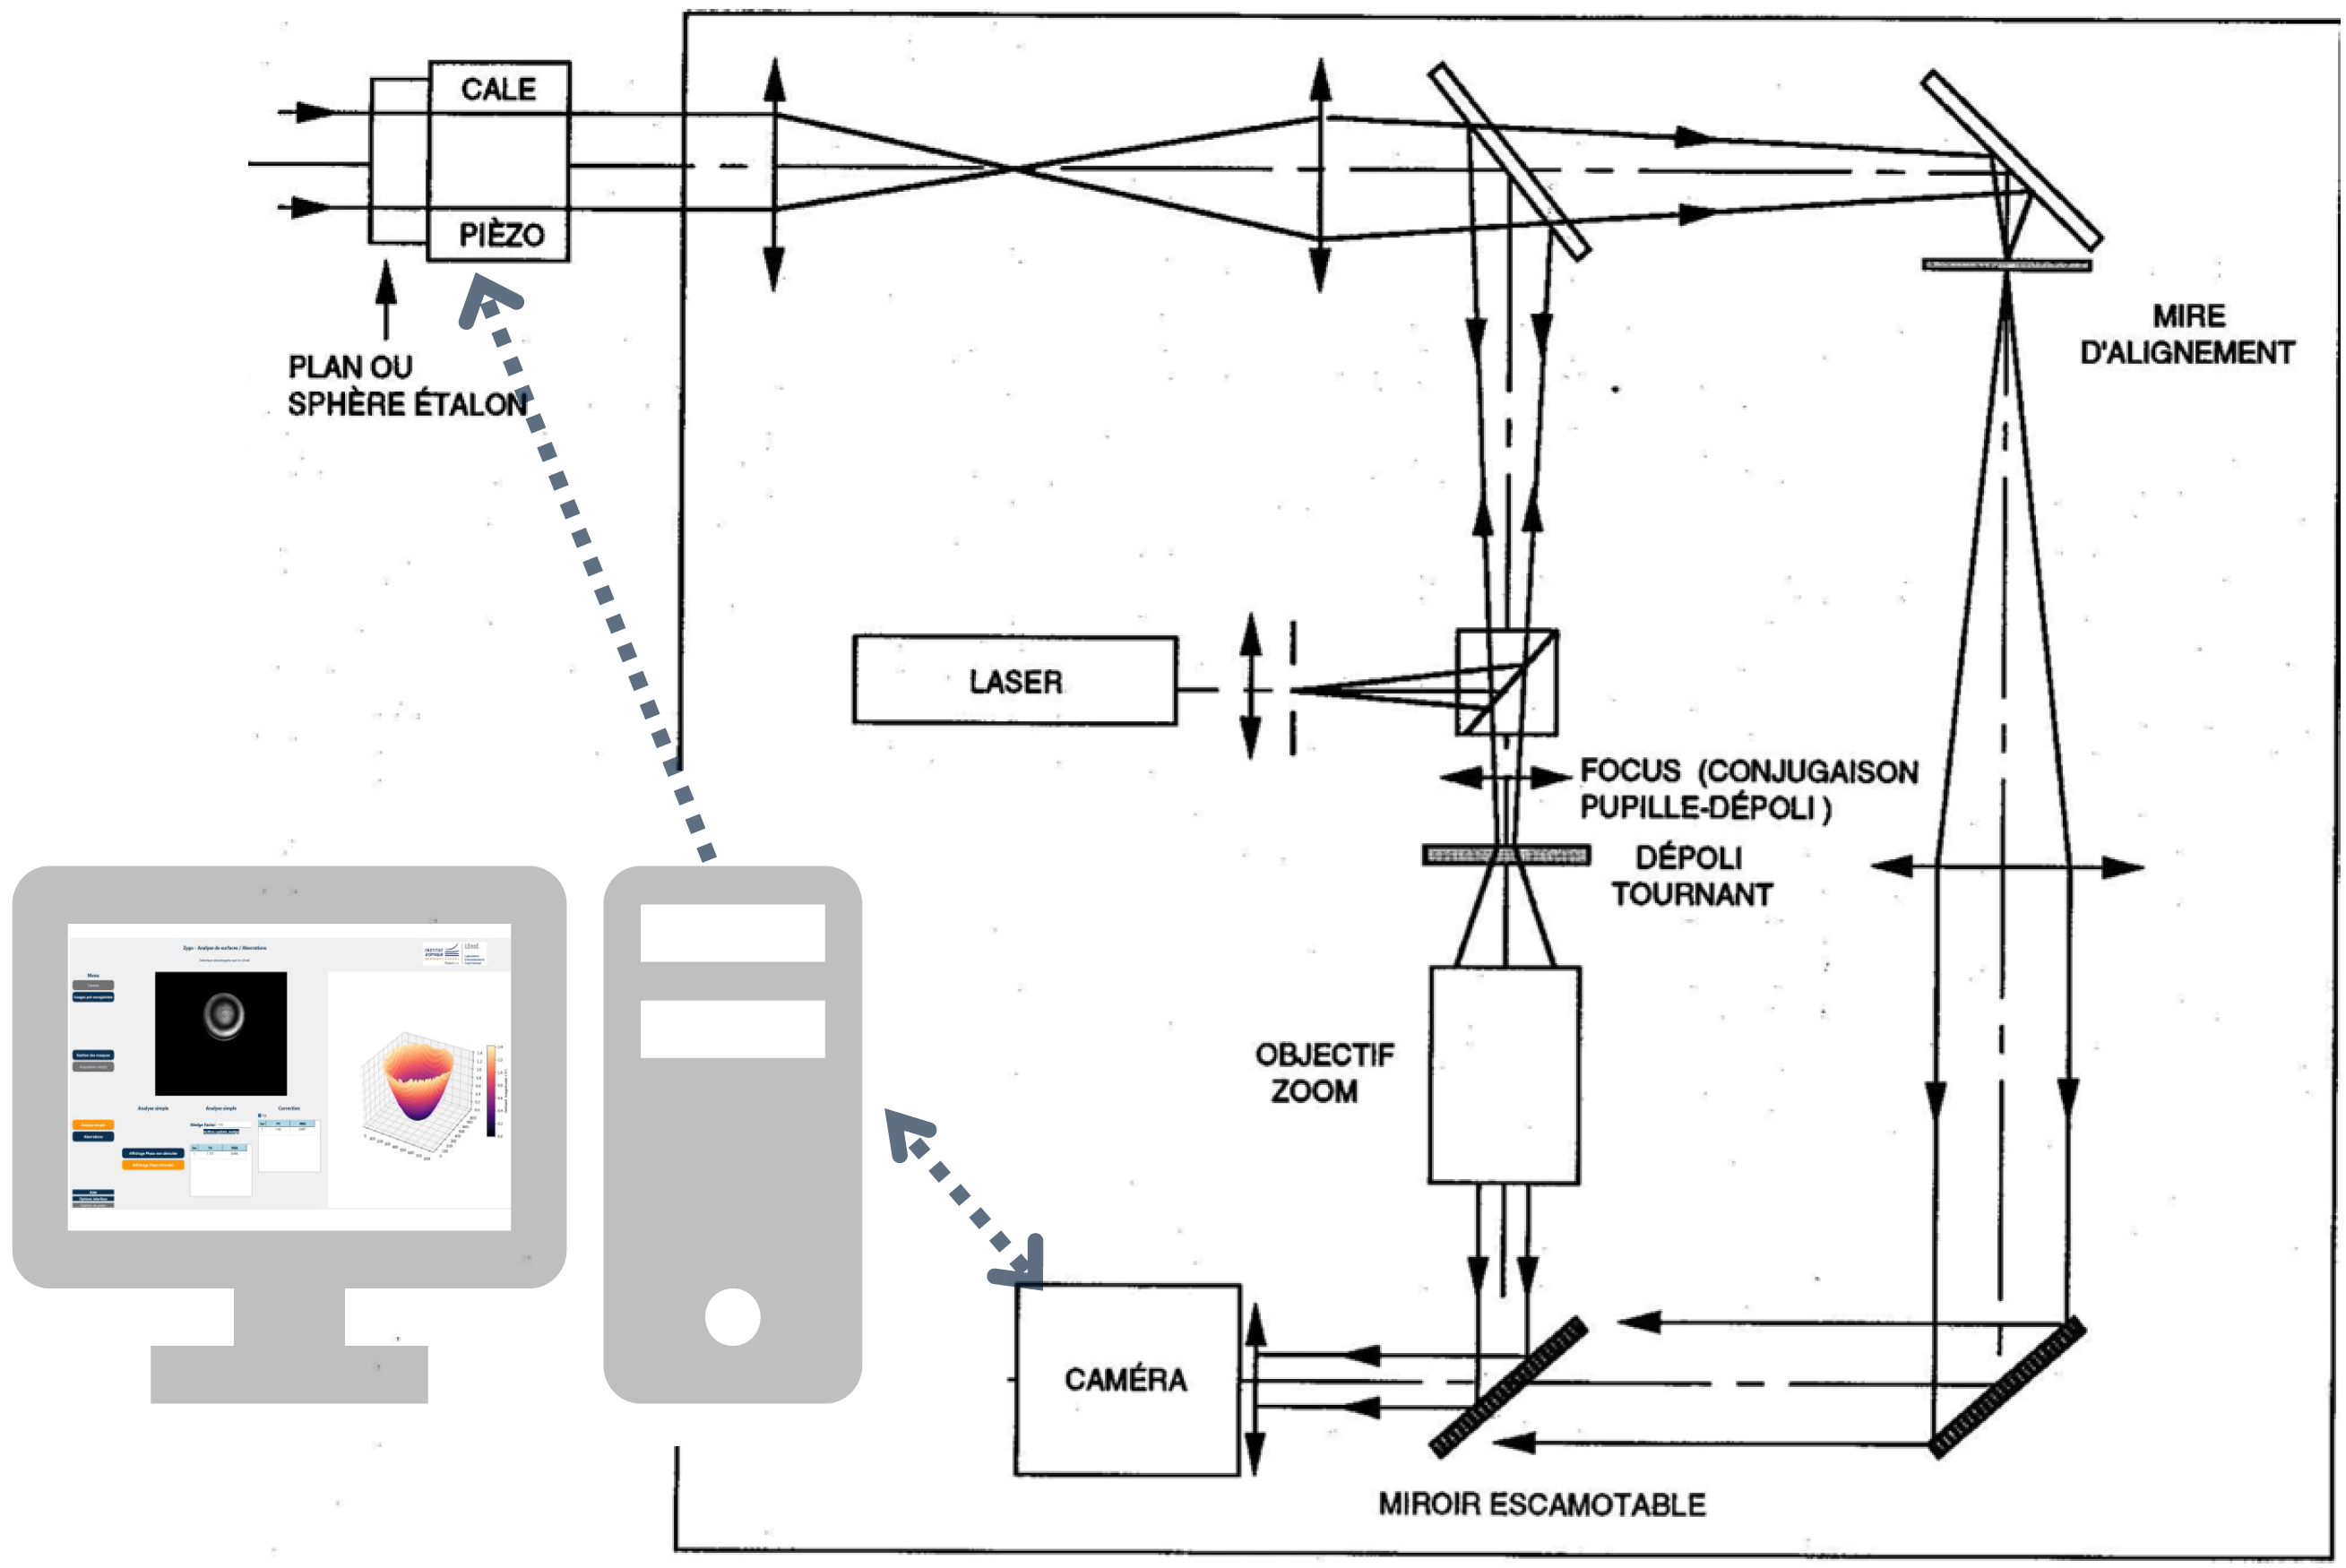
\includegraphics[width=\textwidth]{images/zygo_principe.png}
\end{center}

L'ensemble est piloté par une \textbf{interface de contrôle} présentée dans la suite de ce document.

\clearpage
\section{Précautions}

\begin{tcolorbox}[myboxstyle]
\begin{large}
\begin{center}
Le \textbf{plan de référence} du ZYGO est excellent (quelques $\lambda/100$ RMS), mais évidemment \textbf{très fragile} et \textbf{très onéreux}. C'est la seule pièce très délicate du ZYGO. Prenez-en le plus grand soin ! Ne le touchez jamais ! Placez le support de l'optique à tester loin du plan étalon par sécurité.
\end{center}
\end{large}
\end{tcolorbox}

\medskip

\begin{center}
{\Large \textbf{Replacez TOUJOURS le cache après utilisation.} }
\end{center}

\bigskip


\section{Alignement du système - Miroir plan}

Avant toute utilisation du système, il faudra aligner la partie optique en plaçant le miroir plan parallèle au plan étalon du système de mesure Zygo. Le réglage se fait par \textbf{autocollimation}.

\bigskip

La procédure d'alignement du système est la suivante :

\begin{enumerate}
	\item Placer le \textbf{miroir plan} sur son support, puis en face du \textbf{plan étalon} (sortie du ZYGO) à une distance de quelques dizaine de centimètres.
	\item Positionner le système optique sur la voie de réglage \mbox{\fbox{\textsc{Align}}}.
	\item \textbf{Lancer l'interface du Zygo} : \textsl{\textbf{Start\_Zygo.bat}} sur le bureau de l'ordinateur.
	\item Dans la section \mbox{\fbox{\textsc{Acquisition}}}, cliquer sur \mbox{\fbox{\textsc{Camera}}} puis sur \mbox{\fbox{\textsc{Zoom}}} pour avoir une visualisation en grand écran.
	\item A l'aide des vis de réglage du support du miroir plan, aligner les deux faisceaux lumineux au centre de l'image (au centre de la mire).
\end{enumerate}

Une fois ce réglage effectué, mettre le système optique sur la voie de visualisation \mbox{\fbox{\textsc{View}}}. Vous devriez visualiser des franges d'interférence. 

\begin{center}
	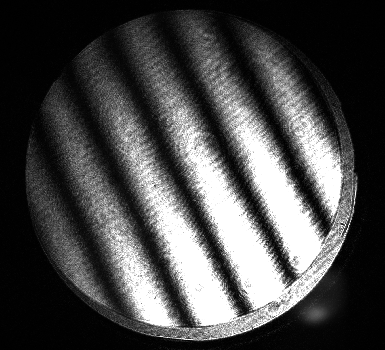
\includegraphics[width=0.3\textwidth]{images/zygo_franges.png}
\end{center}

En modifiant légèrement le réglage précédent du miroir plan, vous devez essayer d'obtenir une teinte la plus plate possible...



% Parties
\cleardoublepage
\ifodd\value{page}\else
  \hbox{}\newpage
\fi

\newpage
%\pagestyle{empty}

\begin{minipage}[c]{.25\linewidth}
	
\includegraphics[width=4cm]{images/Logo-LEnsE.png}
\end{minipage} \hfill
\begin{minipage}[c]{.4\linewidth}

\begin{center}
\vspace{0.3cm}
{\Large \textsc{Interféromètre de ZYGO}}

\medskip

\textbf{\Large \textsc{Mesure de la phase}}

\end{center}
\end{minipage}\hfill

%%%%%%%%%%%%%%%%%%%%%%%%%%%%%%%%%%
\section{Principe de la mesure de la phase}

En interférométrie, l'intensité enregistrée à un point donné dépend de la différence de phase entre deux ondes lumineuses. Pour retrouver cette phase, on modifie intentionnellement la phase d'une des ondes (typiquement à l'aide d'un miroir piézoélectrique), ce qu'on appelle un décalage de phase (\textit{phase shift}), et on enregistre plusieurs images pour reconstituer la phase locale.

L'intensité mesurée en un point est donnée par :

$$I_k = I_0 + I_1 \cdot cos(\Phi + \delta_k)$$

où $I_0$ est l'intensité moyenne,$I_1$ est le contraste, $\Phi$ est la phase que l'on cherche à déterminer et $\delta_k$ est le décalage appliqué à l'étape $k$.

\subsection{Algorithme de Hariharan}

L'algorithme de \textit{phase-shift} (ou décalage de phase) de Hariharan est une méthode d'analyse d'interférogrammes. Il a été développé par P. Hariharan, un pionnier de l'interférométrie, pour permettre une mesure quantitative de la phase avec une précision sub-longueur d'onde.

Cet algorithme a été publié initialiement en 1987 : \textit{P. Hariharan, B. F. Oreb, and T. Eiju, "Digital phase-shifting interferometry: a simple error-compensating phase calculation algorithm," Appl. Opt. 26, 2504-2506 (1987).} Version disponible ici : 


    %Available at: https://opg.optica.org/ao/fulltext.cfm?uri=ao-26-13-2504&id=168363


\subsection{Décalage à 5 pas - intervalle de $\pi/2$}



\begin{figure}[h!]
\centering
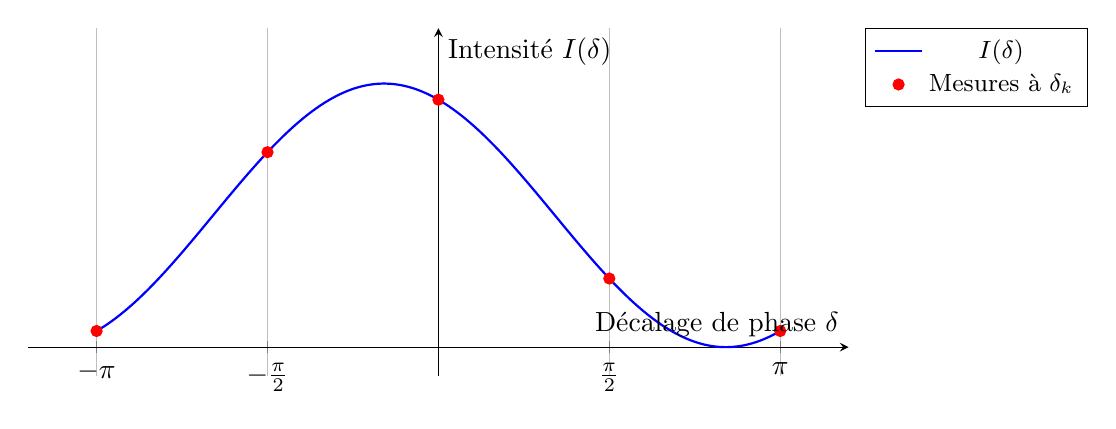
\begin{tikzpicture}
  \begin{axis}[
    domain=-pi:pi,
    samples=300,
    axis lines=middle,
    xlabel={Décalage de phase $\delta$},
    ylabel={Intensité $I(\delta)$},
    xtick={-3.1416, -1.5708, 0, 1.5708, 3.1416},
    xticklabels={$-\pi$, $-\frac{\pi}{2}$, $0$, $\frac{\pi}{2}$, $\pi$},
    ytick=\empty,
    ymin=0, ymax=2.2,
    width=12cm, height=6cm,
    grid=both,
    enlargelimits,
  	legend style={
    		at={(1.02,1)}, anchor=north west,
    		draw=black, fill=white, font=\small
	}
  ]
    % Paramètres de la courbe : I_0 = 1, I_1 = 1, phi = 0.5 rad
    \addplot[blue, thick, domain=-pi:pi] {1 + cos(deg(x + 0.5))};
    \addlegendentry{$I(\delta)$}

    % Points rouges pour les 5 mesures aux décalages multiples de pi/2
    \addplot[only marks, mark=*, red, mark size=2pt]
      coordinates {
        (-pi,   {1 + cos(deg(-pi   + 0.5))})
        (-pi/2, {1 + cos(deg(-pi/2 + 0.5))})
        (0,     {1 + cos(deg(0     + 0.5))})
        (pi/2,  {1 + cos(deg(pi/2  + 0.5))})
        (pi,    {1 + cos(deg(pi    + 0.5))})
      };
    \addlegendentry{Mesures à $\delta_k$}
  \end{axis}
\end{tikzpicture}
\caption{Méthode de décalage de phase à 5 pas avec intervalles de $\pi/2$.}
\end{figure}


\subsection{Reconstruction de la phase}

Prenons cinq images d'interférogrammes $I_1$ à $I_5$ prises aux décalages suivants :
\[
\delta = \{-\pi,\; -\tfrac{\pi}{2},\; 0,\; +\tfrac{\pi}{2},\; +\pi\}.
\]
La phase $\phi$ est alors estimée comme :

\begin{equation}
\phi = \arctan\!\left(
\frac{-2 \bigl(I_2 - I_4\bigr)}
{I_1 - 2I_3 + I_5}
\right)
\end{equation}

\noindent
Cette formule est connue comme l'algorithme de Schwider–Hariharan pour le \textit{5-step $\pi/2$‑shift}.


%%%%%%%%%%%%%%%%%%%%%%%%%%%%%%%%%%%%%%%%%%%%%%%%%%%%%%%%%
%%%%%%%%%%%%%%%%%%%%%%%%%%%%%%%%%%%%%%%%%%%%%%%%%%%%%%%%%
%%%%%%%%%%%%%%%%%%%%%%%%%%%%%%%%%%%%%%%%%%%%%%%%%%%%%%%%%

\newpage
%\pagestyle{empty}

\begin{minipage}[c]{.25\linewidth}
	
\includegraphics[width=4cm]{images/Logo-LEnsE.png}
\end{minipage} \hfill
\begin{minipage}[c]{.4\linewidth}

\begin{center}
\vspace{0.3cm}
{\Large \textsc{Interféromètre de ZYGO}}

\medskip

\textbf{\Large Démarche d'analyse}

\end{center}
\end{minipage}\hfill

%%%%%%%%%%%%%%%%%%%%%%%%%%%%%%%%%%
\section{Démarche d'analyse des interférogrammes}

L'analyse des surfaces ou des aberrations passe par l'acquisition d'images d'interférogrammes par le Zygo, avant une reconstruction de la phase (algorithme de Hariharan) et son déroulement.

A partir de cette phase, il est alors possible d'étudier l'état de surface du système optique à analyser puis de calculer les coefficients de Zernike qui permettent par la suite d'identifier les types d'aberrations présentes dans le système.

\medskip

Les grandes étapes sont décrites succinctement dans la figure suivante :

\begin{tcolorbox}[myboxstyle]
\begin{large}
\begin{center}
L'application se lance par le bouton \textbf{\textsc{Start\_Zygo\_XA.bat}} sur le bureau.
\end{center}
\end{large}
\end{tcolorbox}

\textit{où X est soit 1 (contrôles interférométriques) soit 2 (aberrations).}

\begin{center}
	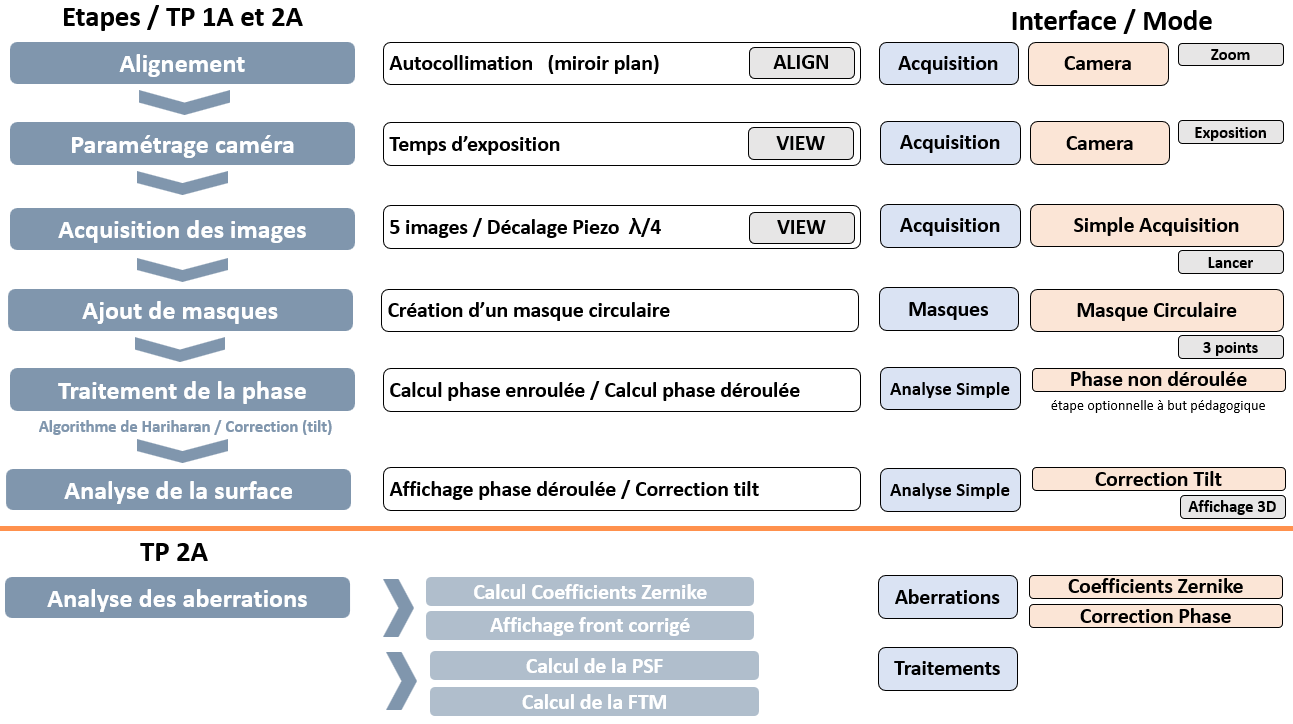
\includegraphics[width=\textwidth]{images/zygo_main_algo.png}
\end{center}

\medskip

Les différents éléments de l'interface de pilotage seront présentés dans la suite de ce document.

\medskip

\medskip

\begin{center}
	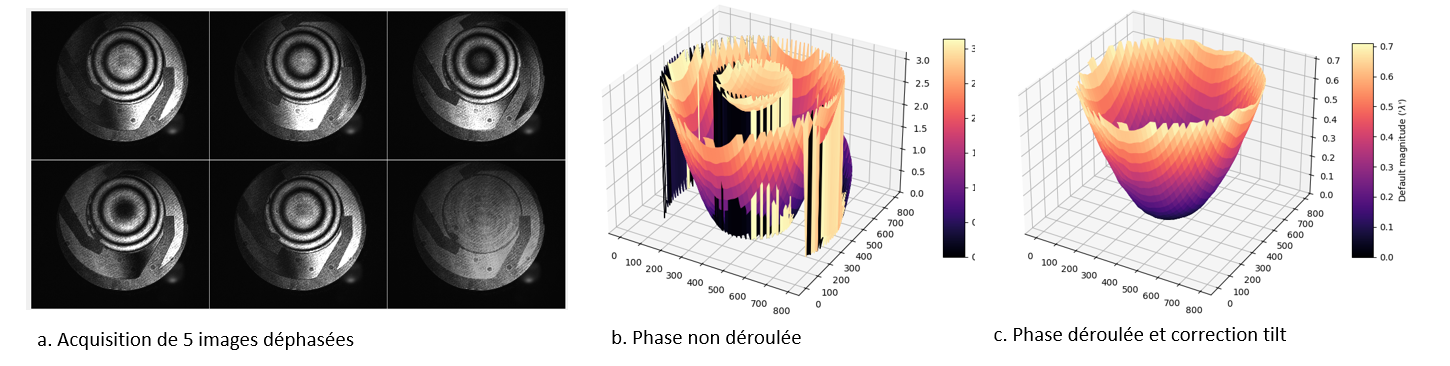
\includegraphics[width=\textwidth]{images/zygo_resultats.png}
\end{center}

\cleardoublepage
\ifodd\value{page}\else
  \hbox{}\newpage
\fi

\newpage
%\pagestyle{empty}

\begin{minipage}[c]{.25\linewidth}
	
\includegraphics[width=4cm]{images/Logo-LEnsE.png}
\end{minipage} \hfill
\begin{minipage}[c]{.4\linewidth}

\begin{center}
\vspace{0.3cm}
{\Large \textsc{Interféromètre de ZYGO}}

\medskip

\textbf{\Large IHM - \textsc{Généralités}}

\end{center}
\end{minipage}\hfill

%%%%%%%%%%%%%%%%%%%%%%%%%%%%%%%%%%
\section{Structure de l'interface}

L'interface de contrôle de l'interféromètre de Zygo se présente ainsi :

\begin{center}
	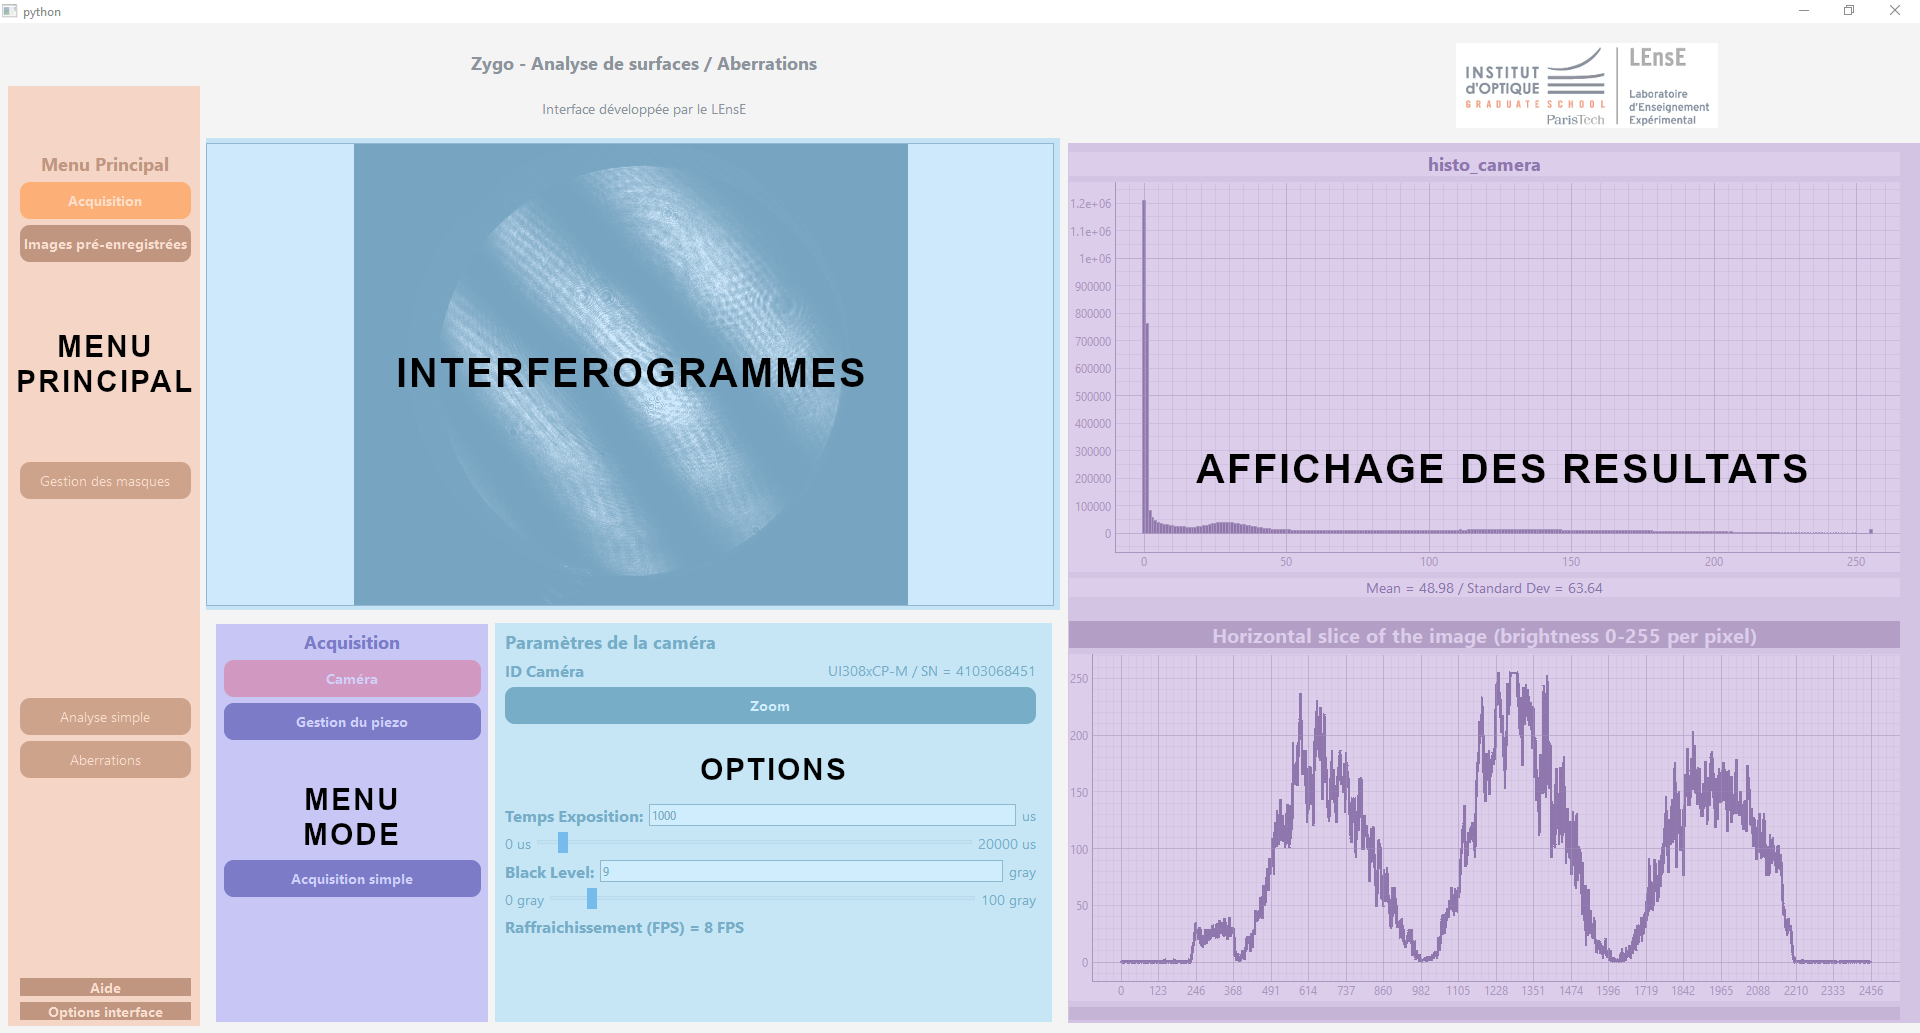
\includegraphics[width=\textwidth]{images/zygo_ihm_structure.png}
\end{center}


Il est possible d'accéder aux différentes sections de l'application par le \textbf{\textsc{menu principal}}. Chaque section de ce menu correspond à une des étapes de l'analyse.

\medskip

La partie \textbf{\textsc{Menu Mode}} affiche le menu spécifique à la section choisie dans le menu principal.

La partie \textbf{\textsc{Options}} affiche les options spécifiques à la sous-section choisie dans le menu mode.

\medskip

La partie \textbf{\textsc{Interférogrammes}} affiche (dans la plupart des étapes) l'interférogramme de référence.

La partie \textbf{\textsc{Affichage des résultats}} affiche les résultats des différents calculs proposés dans chaque section.

\medskip

Certaines options entraînent des phases de calcul un peu longues (affichage 3D, PSF...).

\bigskip


\begin{tcolorbox}[myboxstyle]
\begin{large}
\begin{center}
L'application se lance depuis le bureau par le bouton 

\begin{itemize}
	\item \textbf{\textsc{Start\_Zygo\_1A.bat}}  pour les TP sur le contrôle interférométrique
	\item \textbf{\textsc{Start\_Zygo\_2A.bat}}  pour les TP sur les aberrations
\end{itemize}

 .
\end{center}
\end{large}
\end{tcolorbox}

\bigskip

\textit{Une procédure d'installation est également proposée à la fin de ce document...}


\newpage
%%%%%%%%%%%%%%%%%%%%%%%%%%%%%%%%%%
\section{Structure de l'application}

\cleardoublepage
\ifodd\value{page}\else
  \hbox{}\newpage
\fi

\newpage
%\pagestyle{empty}

\begin{minipage}[c]{.25\linewidth}
	
\includegraphics[width=4cm]{images/Logo-LEnsE.png}
\end{minipage} \hfill
\begin{minipage}[c]{.4\linewidth}

\begin{center}
\vspace{0.3cm}
{\Large \textsc{Interféromètre de ZYGO}}

\medskip

\textbf{\Large IHM - \textsc{Acquisition}}

\end{center}
\end{minipage}\hfill

%%%%%%%%%%%%%%%%%%%%%%%%%%%%%%%%%%
%%%%%%%%%%%%%%%%%%%%%%%%%%%%%%%%%%
\section{Acquisition d'une série d'interférogrammes}

La première étape avant de pouvoir analyser l'état de surface des optiques est l'\textbf{acquisition des interférogrammes} à différentes positions.

Cette étape se fait dans la partie \mbox{\fbox{\textbf{\textsc{Acquisition}}}} de l'application.

\medskip

Cette section regroupe les sous-mode suivant :

\begin{description}
	\item[\mbox{\fbox{Caméra}}] qui permet de modifier le temps d'exposition et le niveau de noir de la caméra Basler du système
	\item[\mbox{\fbox{Gestion du piezo}}] qui permet de valider le fonctionnement de la cale piézoélectrique
	\item[\mbox{\fbox{Acquisition Simple}}] qui permet de lancer une nouvelle acquisition d'interférogramme (5 images déphasées de $\lambda/4$.
\end{description}


%%%%%%%%%%%%%%%%%%%%%%%%%%%%%%%%%%
\subsection{Caméra}

La section \mbox{\fbox{\textsc{\textbf{Caméra}}}} permet de lancer la \textbf{visualisation de l'interférogramme} (en mode \textsc{View}).

Un \textbf{histogramme} ainsi qu'une \textbf{coupe au centre de l'image} sont affichés dans la partie de droite. 

\medskip

Il est possible de régler le \textbf{temps d'exposition} et le \textbf{niveau de noir} (offset des pixels) de la caméra. 

\medskip

Le \textbf{niveau de noir} doit être réglé pour que les franges sombres ne soient pas écrêtées vers le bas (autour de 0) sur la coupe tout en maintenant un niveau proche de 0 en terme de luminisité.

Le \textbf{temps d'exposition} doit être réglé pour que les franges claires ne soient pas écrêtées vers le haut (autour de 255) sur la coupe tout en garantissant la meilleure dynamique possible sur la caméra.

\medskip


\begin{center}
	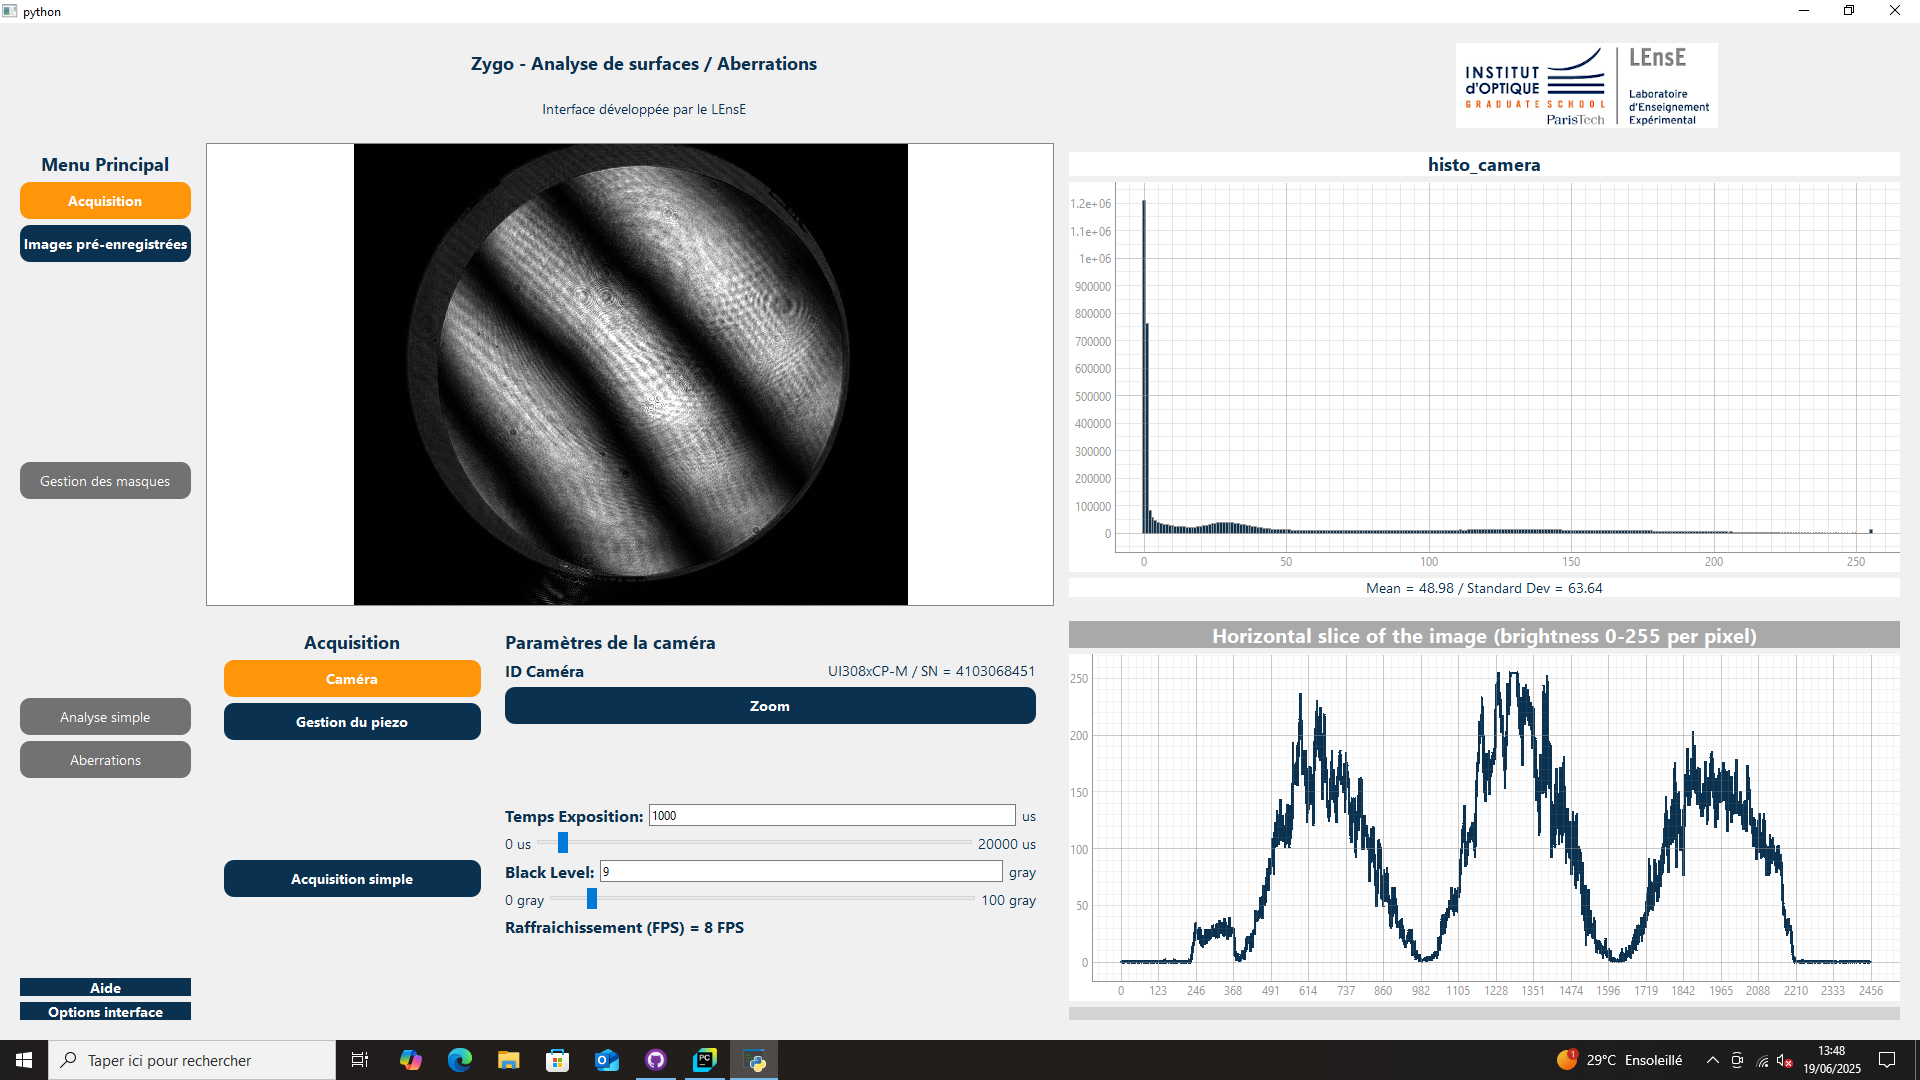
\includegraphics[width=0.9\textwidth]{images/zygo_acquisition_camera.png}
\end{center}

\newpage

%%%%%%%%%%%%%%%%%%%%%%%%%%%%%%%%%%
\subsection{Acquisition Simple}

La section \mbox{\fbox{\textsc{\textbf{Acquisition Simple}}}} permet de lancer l'\textbf{acquisition de 5 interférogrammes}.

\medskip

Il faut cliquer sur l'un des deux boutons \mbox{\fbox{\textsc{Lancer l'acquisition}}}.

Le \textbf{premier bouton} supprime tous les masques en mémoire.

Le \textbf{second bouton} conserve l'ensemble des masques déjà pré-établis.

\medskip

Une barre de progression permet de connaître l'état d'avancement de l'acquisition. Cette phase dure quelques secondes.

\bigskip

Lorsque l'acquisition est terminée, une série de 6 images s'affiche dans la partie de droite : les 5 premières images correspondent à chaque interférogramme déphasé de $\lambda/4$ et la dernière (en bas à droite) correspond à la somme des 4 premières.

La dernière image doit montrer une teinte quasiment plate dans la zone d'étude.


\begin{center}
	
\includegraphics[width=0.9\textwidth]{images/zygo_acquisition_simple.png}
\end{center}

%%%%%%%%%%%%%%%%%%%%%%%%%%%%%%%%%%
\subsection{Gestion de la cale piézoélectrique}

La section \mbox{\fbox{\textsc{\textbf{Gestion du piezo}}}} permet de \textbf{modifier la tension appliquée à la cale piézoélectrique}, permettant de changer le chemin optique et ainsi déplacer les franges de l'interférogramme.

IMAGES pour V=1V, V=2V, V=3V ?


\cleardoublepage
\ifodd\value{page}\else
  \hbox{}\newpage
\fi

\newpage
%\pagestyle{empty}

\begin{minipage}[c]{.25\linewidth}
	
\includegraphics[width=4cm]{images/Logo-LEnsE.png}
\end{minipage} \hfill
\begin{minipage}[c]{.4\linewidth}

\begin{center}
\vspace{0.3cm}
{\Large \textsc{Interféromètre de ZYGO}}

\medskip

\textbf{\Large IHM - \textsc{Masques}}

\end{center}
\end{minipage}\hfill

%%%%%%%%%%%%%%%%%%%%%%%%%%%%%%%%%%
%%%%%%%%%%%%%%%%%%%%%%%%%%%%%%%%%%
\section{Création d'un masque}

La seconde étape avant de pouvoir analyser l'état de surface des optiques est de \textbf{définir un masque sur la zone d'étude}.

Cette étape se fait dans la partie \mbox{\fbox{\textbf{\textsc{Gestion des Masques}}}} de l'application.

\medskip

Cette section permet de :

\begin{itemize}
	\item \textbf{gérer les masques déjà présents} (section \textbf{Affichage des masques}) : suppression, sélection, inversion... 
	\item \textbf{ajouter un nouveau masque} (boutons \textbf{Masque Circulaire}...) d'un certain type
\end{itemize}

\begin{center}
	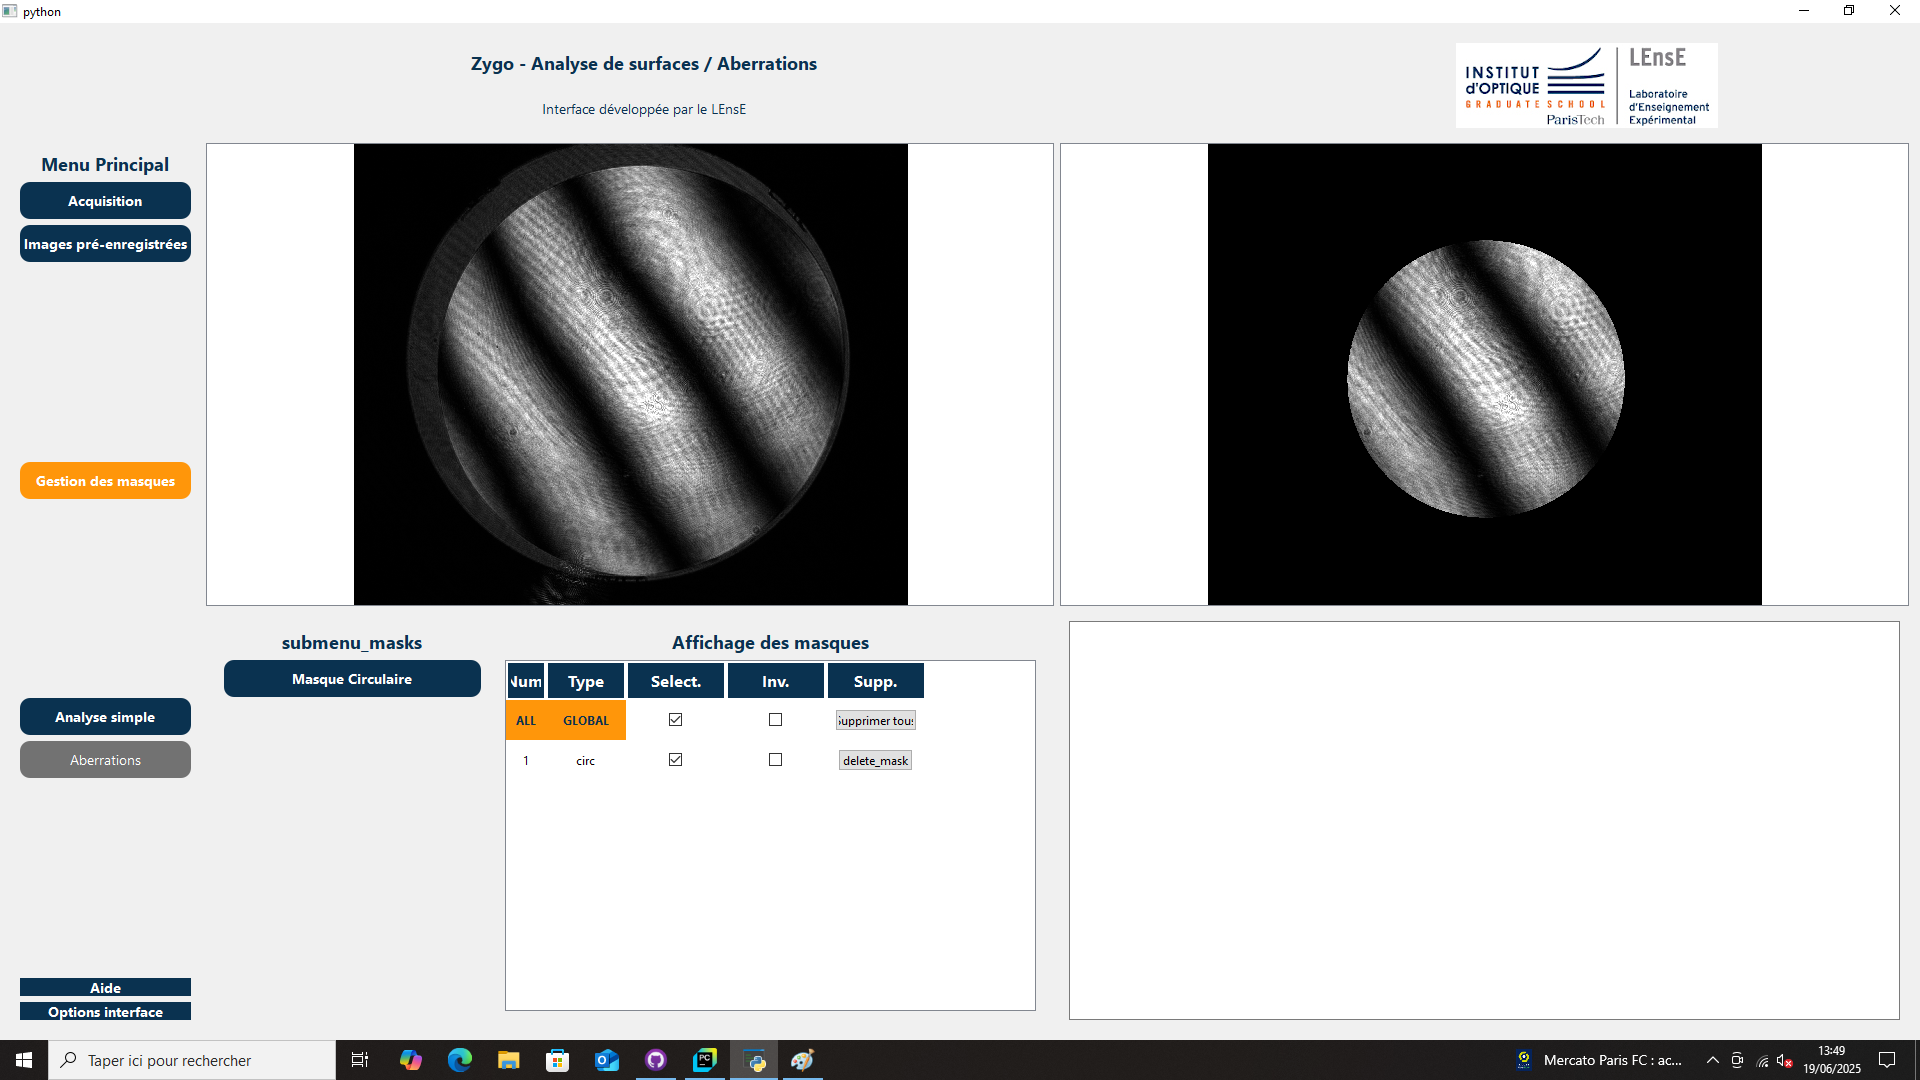
\includegraphics[width=0.9\textwidth]{images/zygo_masques.png}
\end{center}

\subsection{Ajout d'un nouveau masque}

Vous devez cliquer sur l'un des boutons \mbox{\fbox{\textbf{\textsc{Masque ...}}}}, en fonction du type de masque voulu.

\bigskip

Lors de l'ajout d'un masque, une nouvelle fenêtre s'ouvre.

Les \textbf{masques circulaires} nécessitent de choisir \textbf{3 points} dans l'image. Le cercle sera ensuite calculé pour passer par ces trois points.


\begin{tcolorbox}[myboxstyle]
\begin{large}
\begin{center}
Pour l'étude des \textbf{aberrations}, un seul masque est nécessaire. 

Il doit être de type \textbf{circulaire}.
\end{center}
\end{large}
\end{tcolorbox}



\end{document}


